\documentclass[10pt,a4paper]{article}
\usepackage[utf8]{inputenc}
\usepackage[english]{babel}
\usepackage{amsmath}
\usepackage{amsfonts}
\usepackage{amssymb}
\usepackage{blindtext} % for random texts
\usepackage{graphicx} % to show images
\usepackage{booktabs} % for tables
\usepackage[table,xcdraw]{xcolor}
\usepackage{hyperref} % to create hyperlinks in  sections, figures...
\hypersetup{
    colorlinks=true,
    linkcolor=blue,
    filecolor=magenta,      
    urlcolor=cyan,
    pdftitle={Overleaf Example},
    pdfpagemode=FullScreen,
    }
    
\usepackage[left=2cm,right=2cm,top=2cm,bottom=2cm]{geometry} % changes the page margins

\title{My first ~\LaTeX~ document}
\author{Camila Celeste RIBA PEREYRA}
\date{\today}

%environments go from \begin to \end

\begin{document}

\maketitle
\tableofcontents %in big files needs to be compiled twice in order to be updated.

\section{Basic text configuration}

Hello world!

Different lines can be written separately in different cmd lines.
In the document will look like one paragraph.

To add another paragraph a blank line is needed.

\vspace{1cm} Vspace is a command to separate the upper part of the paragraph as wished.

\noindent Indentation can be avoided with \emph{noindent}.

\section{How to add formulas}
To write inline maths add the formula inside dollar signs:
$\rho = 500 \Omega * m$ .

To write formulas in single line, standalone, put two dollars in the upper and down rows.

$$
T = \dfrac{1}{\rho}
$$

\noindent We can enumerate objects or formulas like a list: 

\begin{enumerate}
\item  $T = \dfrac{1}{\rho}$
\item  ${\rho} = \dfrac{1}{T}$
\end{enumerate}

\noindent Or we can add numeration to the equations:
\begin{equation}
T = \dfrac{1}{\rho}
\end{equation}
\begin{equation}
{\rho} = \dfrac{1}{T}
\label{eq:personalised label}
\end{equation}


\section{Figures and plots}
We can add figures that are inside the same folder as the LaTeX document, like figure \ref{plot1} on page \pageref{plot1}
\begin{figure}
	\begin{center}
		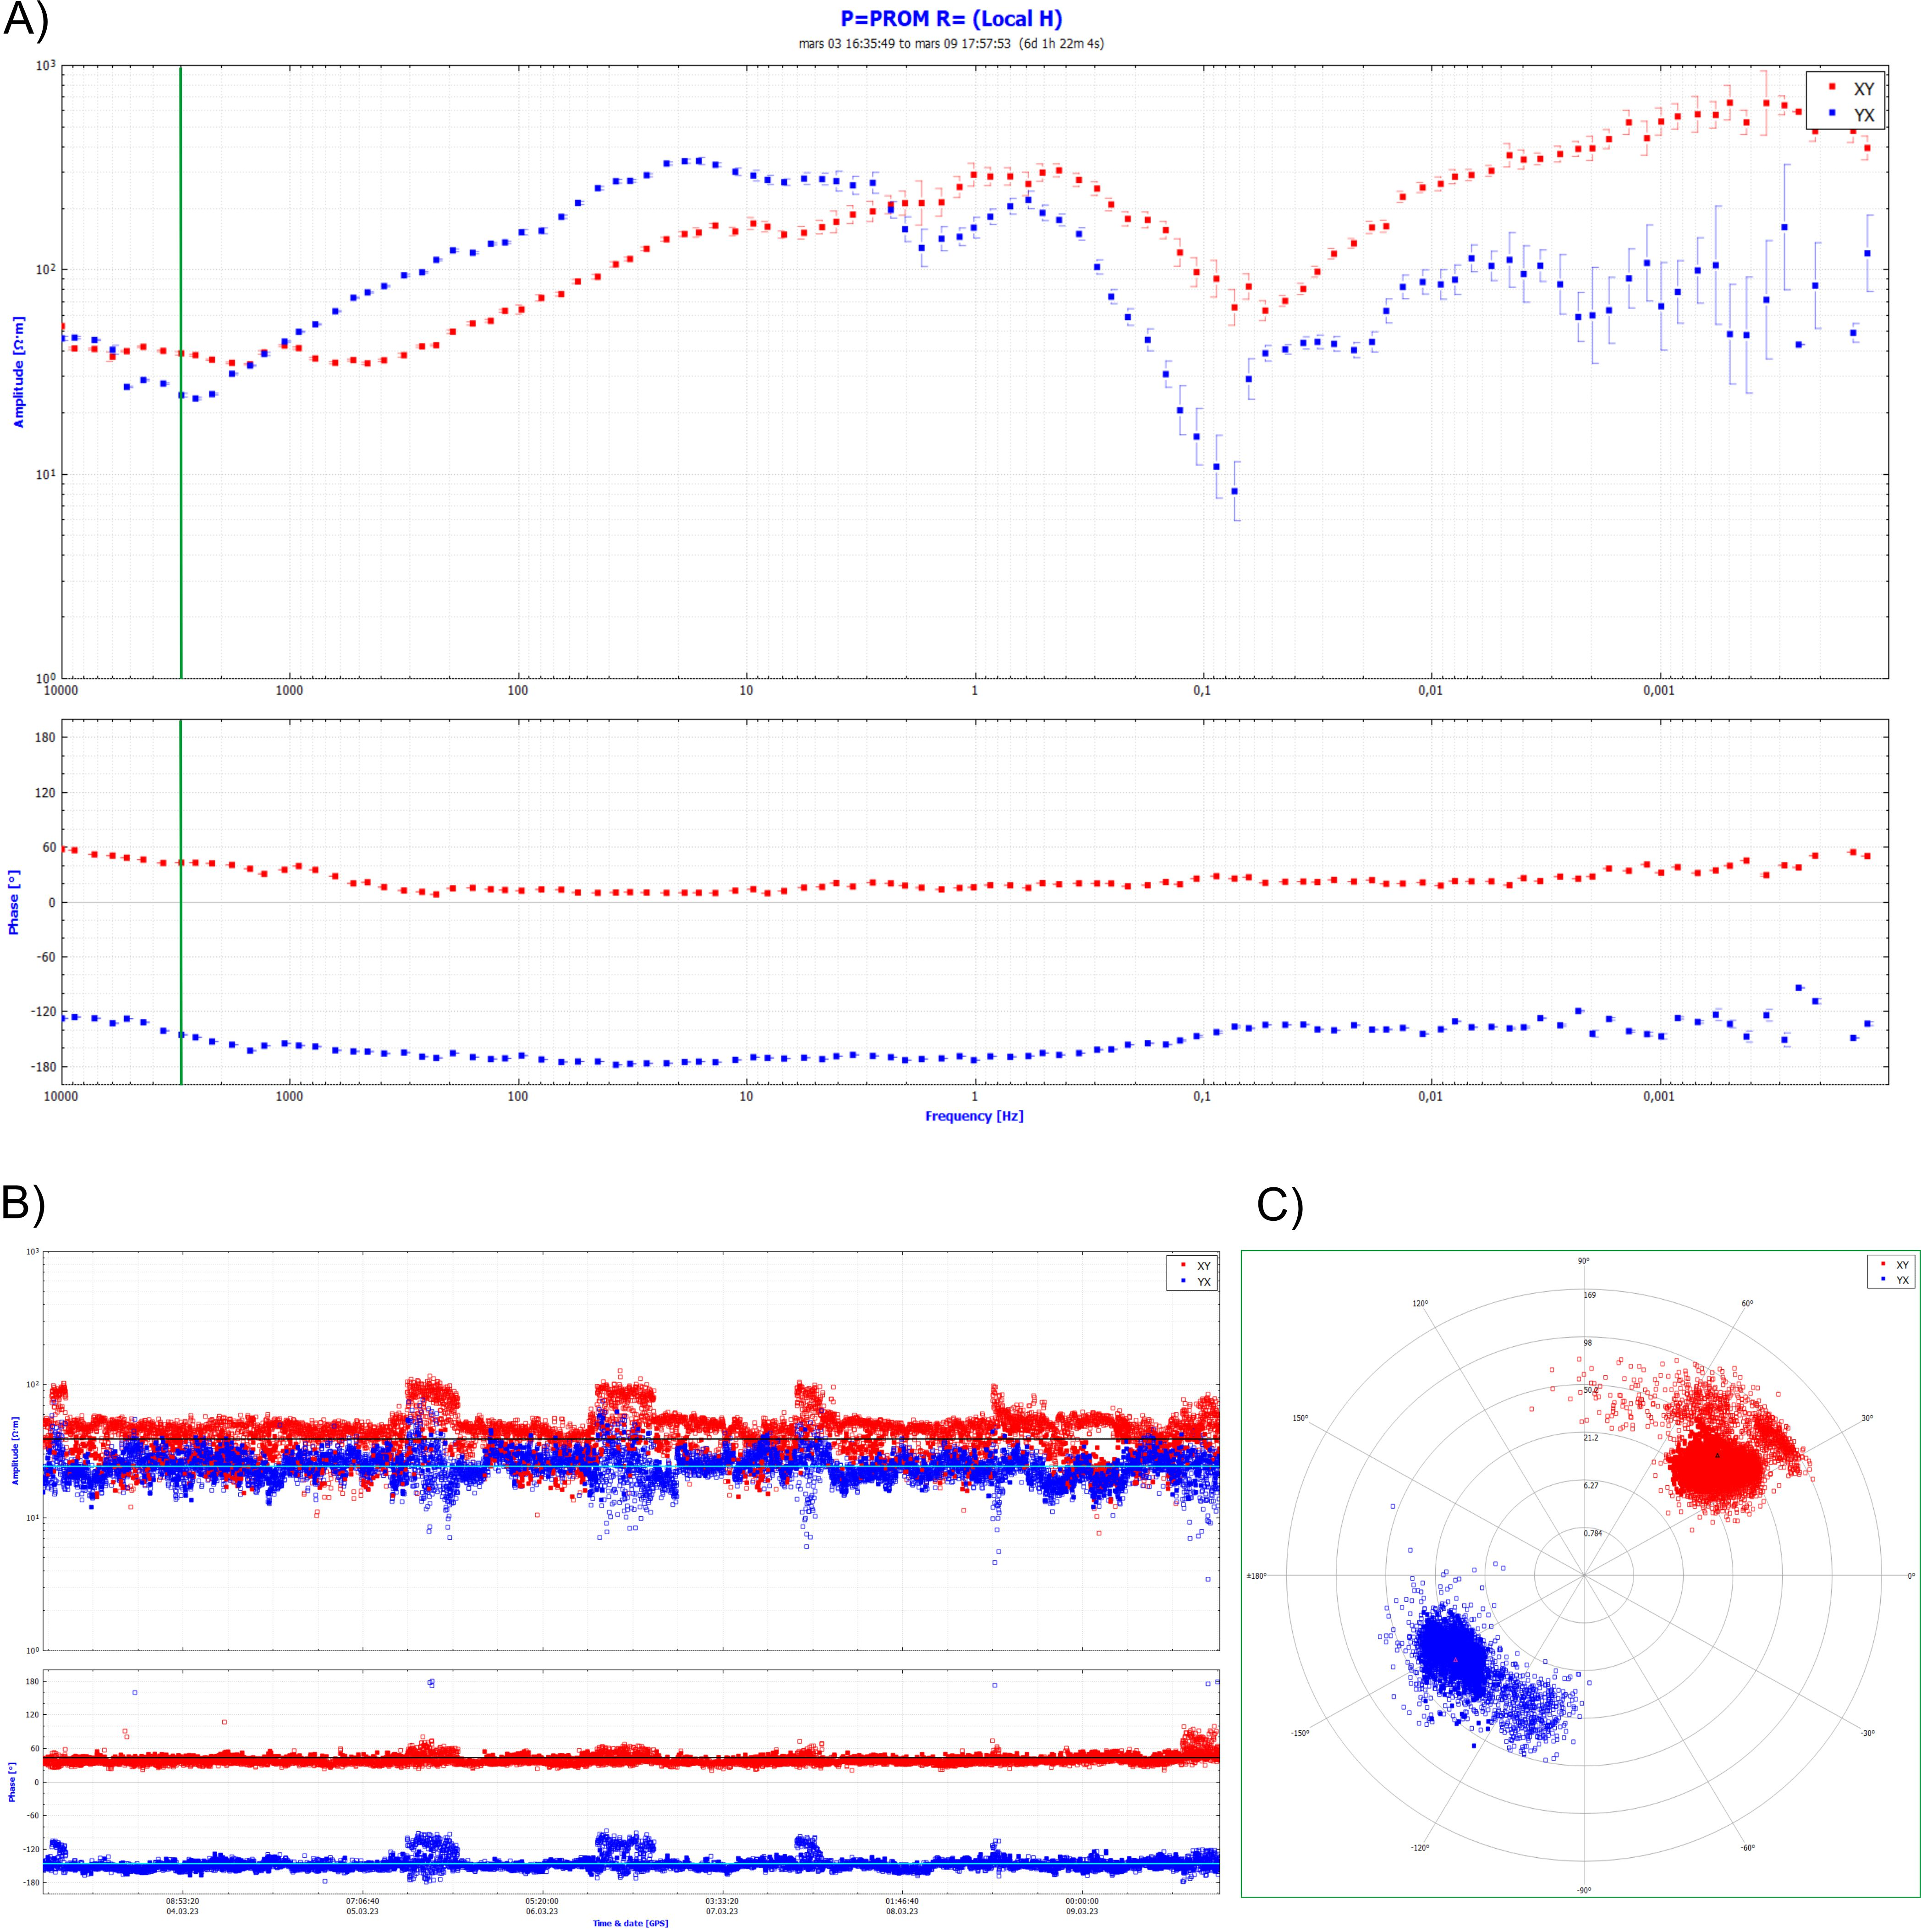
\includegraphics[width = 14cm]{phd-isterre-poster-2023-fig.jpg}
	\end{center}
	\caption{Example of caption.}
	\label{plot1} %used for hyperlink figures
\end{figure}



\section{Tabulars and tables}
\vspace{1cm}
\begin{tabular}{|c|c|c|}
\hline %horizontal separator
\textbf{Frequency} & \textbf{Phase} & \textbf{Apparent resistivity} \\ %& is the separator
\hline
256Hz & 48-140° & 2156 $\Omega$ m \\
\hline
\end{tabular}

\vspace{1cm}
\begin{tabular}{ccc}
\toprule
    \textbf{Animal} & \textbf{Size} & \textbf{Weight} \\
    \midrule
    Rabbit          & Small         & $1$ kg          \\
    Rabbit          & Small         & $1$ kg          \\
    Rabbit          & Small         & $1$ kg          \\
    Rabbit          & Small         & $1$ kg          \\
    \bottomrule
\end{tabular}
\vspace{1cm}

\subsection{Using Tablesgenerator}

Using \url{www.tablesgenerator.com}.

\vspace{1cm}

\begin{tabular}{@{}ccc@{}}
    \toprule
    \cellcolor[HTML]{6665CD}Name                    & \cellcolor[HTML]{6665CD}Here                       & There                      \\ \midrule
    \rowcolor[HTML]{6665CD}
    \multicolumn{1}{|c|}{\cellcolor[HTML]{6665CD}1} & \multicolumn{2}{c|}{\cellcolor[HTML]{6665CD}08:15}                              \\ \midrule
    \multicolumn{1}{|c|}{2}                         & \multicolumn{1}{c|}{13:30}                         & \multicolumn{1}{c|}{17:30} \\ \midrule
    \multicolumn{1}{l}{2bis}                        & \multicolumn{1}{l}{14:30}                          & \multicolumn{1}{l}{18:30}  \\ \bottomrule
\end{tabular}


\section{Bibliography}
We can cite articles with \emph{cite}, as \cite{Smai2020} and \cite{Chave2012}. Then we can add the references using a bib file created with JabRef.

\bibliography{bibliography.bib}
\bibliographystyle{plain}


\end{document}
